
\chapter{实验结果}
\label{cha:experiment}

在本章中,我们完整地展示了 F2000 模式分量的代码生成、编译、运行、数据分析等步骤。

\section{配置文件}

\usetikzlibrary{trees}
\tikzstyle{every node}=[draw=black,thick,anchor=west]
\tikzstyle{selected}=[draw=red,fill=red!30]
\tikzstyle{optional}=[dashed,fill=gray!50]

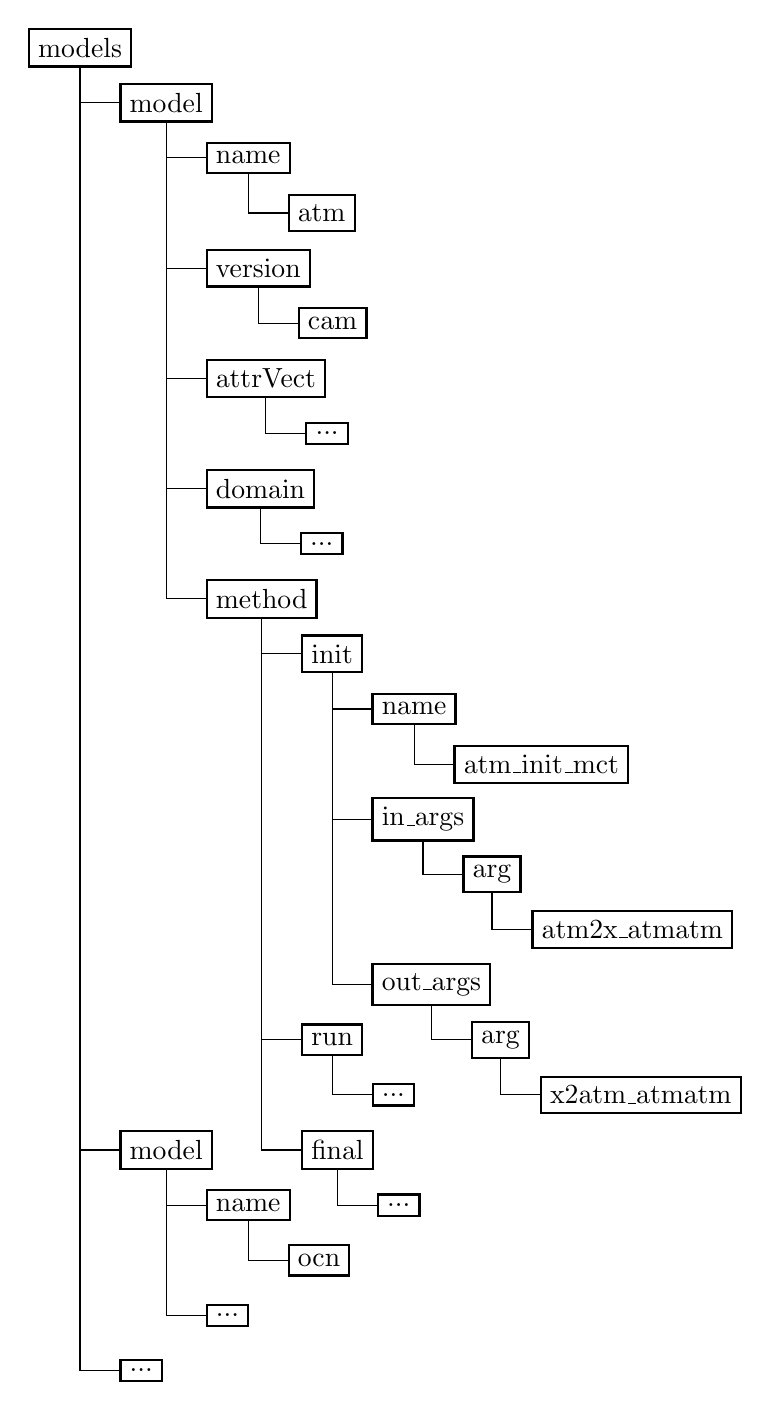
\begin{tikzpicture}[%
  grow via three points={one child at (0.5,-0.7) and
  two children at (0.5,-0.7) and (0.5,-1.4)},
  edge from parent path={(\tikzparentnode.south) |- (\tikzchildnode.west)}]
  \node{models}
  child { node {model}
    child { node {name}
      child {node {atm}}
    }
    child [missing] {}
    child { node {version}
      child {node {cam}}
    }
    child [missing] {}
    child { node {attrVect}
      child {node {...}}
    }
    child [missing] {}    
    child { node {domain}
      child {node {...}}
    }
    child [missing] {}    
    child { node {method}
      child {node {init}
        child { node {name}
        	child { node {atm\_init\_mct}}
        }
        child [missing] {}
        child { node {in\_args}
          child { node {arg}
            child { node {atm2x\_atmatm}}
          }
        }
        child [missing] {}
        child [missing] {}
        child { node {out\_args}
          child { node {arg}
            child { node {x2atm\_atmatm}}
          }
        }
        child [missing] {}
        child [missing] {}
      }
      child [missing] {}
      child [missing] {}
      child [missing] {}
      child [missing] {}
      child [missing] {}
      child [missing] {}
      child {node {run}
        child { node {...} }
      }
      child [missing] {}    
      child {node {final}
        child { node {...} }
      }
      child [missing] {}    
    }
  }
  child [missing] {}    
  child [missing] {}    
  child [missing] {}    
  child [missing] {}    
  child [missing] {}    
  child [missing] {}    
  child [missing] {}    
  child [missing] {}    
  child [missing] {}    
  child [missing] {}    
  child [missing] {}    
  child [missing] {}    
  child [missing] {}    
  child [missing] {}    
  child [missing] {}    
  child [missing] {}    
  child [missing] {}    
  child [missing] {}    
  child { node {model}
    child { node {name}
      child { node {ocn} }
    }
    child [missing] {}
    child { node {...} }
  }
  child [missing] {}
  child [missing] {}
  child [missing] {}
  child {node {...}};
\end{tikzpicture}


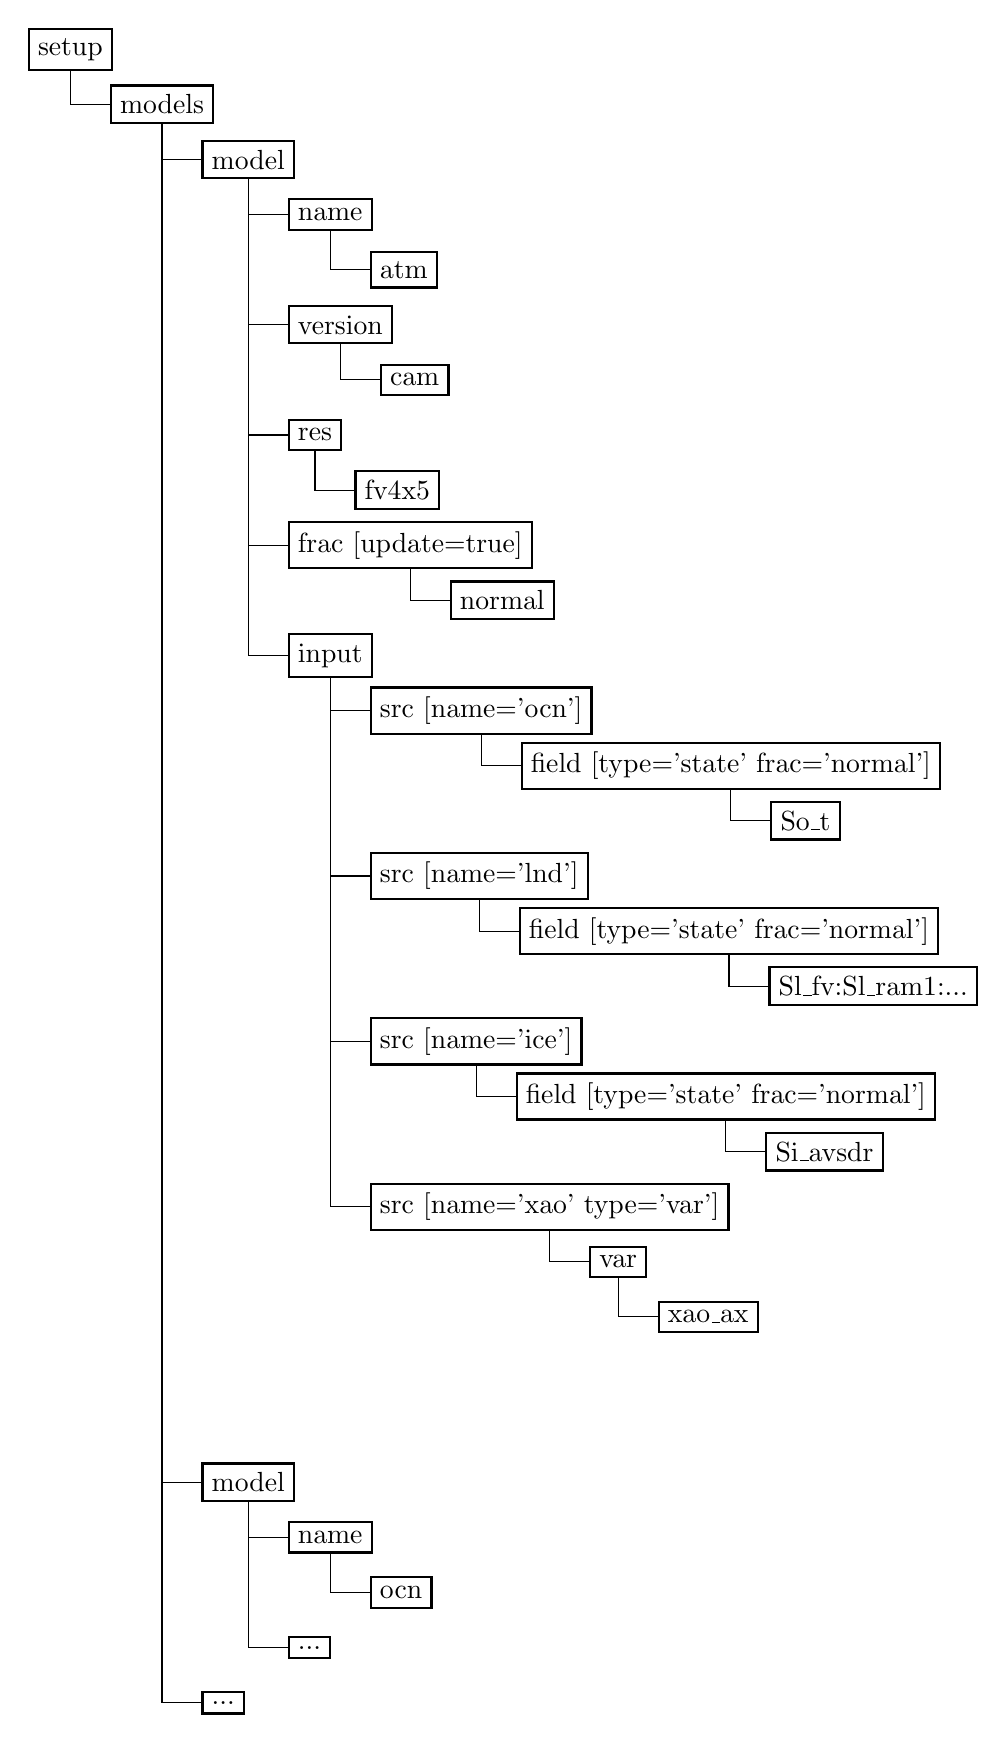
\begin{tikzpicture}[%
  grow via three points={one child at (0.5,-0.7) and
  two children at (0.5,-0.7) and (0.5,-1.4)},
  edge from parent path={(\tikzparentnode.south) |- (\tikzchildnode.west)}]
  \node {setup}
    child { node {models} 
      child { node {model}
        child { node {name}
          child { node {atm} }
        }
        child [missing] {}
        child { node {version}
          child { node {cam} }
        }
        child [missing] {}    		
        child { node {res}
          child { node {fv4x5} }
        }
        child [missing] {}
        child { node {frac [update=true]}
          child { node {normal} }
        }
        child [missing] {}
        child { node {input}
          child { node {src [name='ocn']} 
          	child { node {field [type='state' frac='normal']}
          	  child {node {So\_t}}
          	}
          	child [missing] {}          	
          }
          child [missing] {}
          child [missing] {}
          child { node {src [name='lnd']} 
          	child { node {field [type='state' frac='normal']}
          	  child {node {Sl\_fv:Sl\_ram1:...}}
          	}
          	child [missing] {}          	
          }
          child [missing] {}
          child [missing] {}
          child { node {src [name='ice']} 
          	child { node {field [type='state' frac='normal']}
          	  child {node {Si\_avsdr}}
          	}
          	child [missing] {}          	
          }
          child [missing] {}
          child [missing] {}          
          child { node {src [name='xao' type='var']} 
          	child { node {var}
          	  child {node {xao\_ax}}
          	}
          	child [missing] {}      	
          }
          child [missing] {}
          child [missing] {}        }
        child [missing] {}
      }
      child [missing] {}
      child [missing] {}
      child [missing] {}
      child [missing] {}
      child [missing] {}
      child [missing] {}
      child [missing] {}
      child [missing] {}
      child [missing] {}
      child [missing] {}
      child [missing] {}
      child [missing] {}
      child [missing] {}
      child [missing] {}
      child [missing] {}
      child [missing] {}
      child [missing] {}
      child [missing] {}
      child [missing] {}
      child [missing] {}
      child [missing] {}
      child [missing] {}
      child [missing] {}
      child { node {model}
        child { node {name}
          child { node {ocn} }
        }
        child [missing] {}
        child { node {...} }
      }
      child [missing] {}
      child [missing] {}
      child [missing] {}
      child { node {...} } 
    };
\end{tikzpicture}

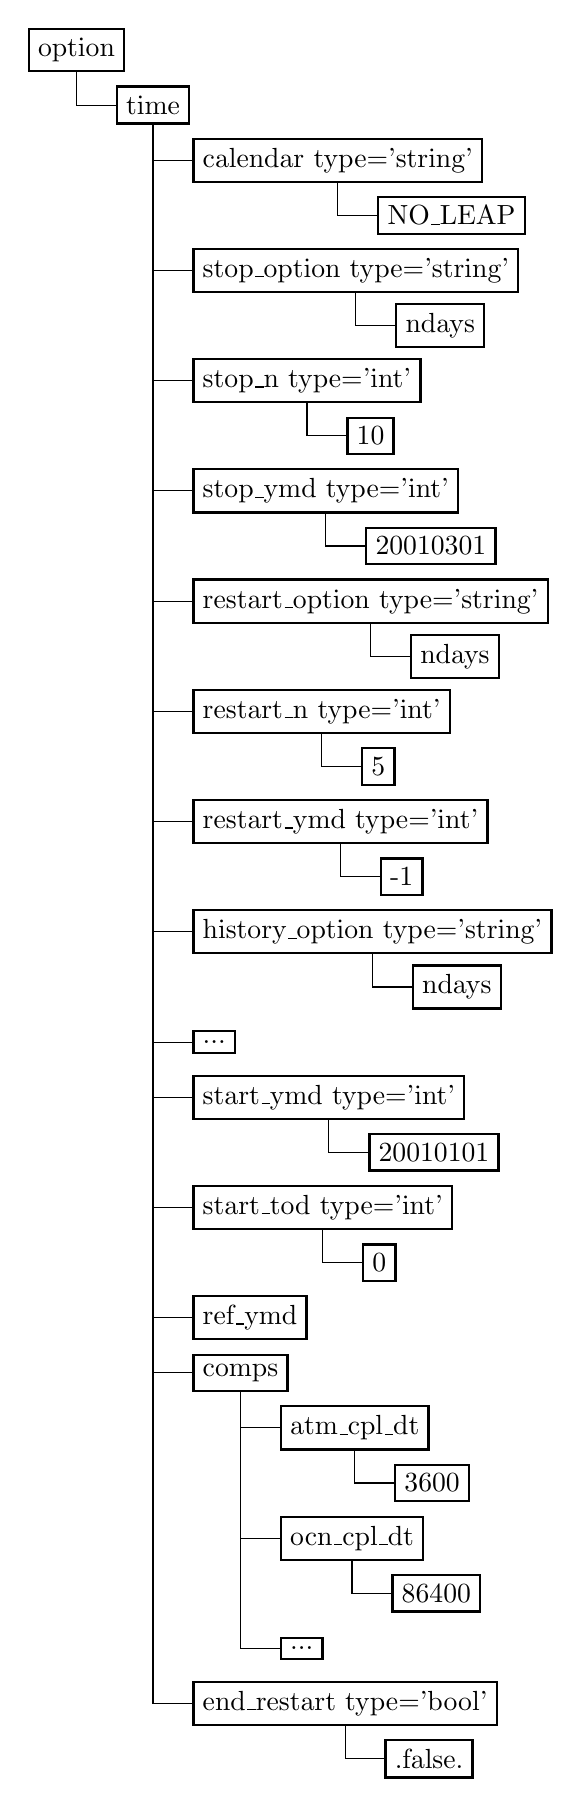
\begin{tikzpicture}[%
  grow via three points={one child at (0.5,-0.7) and
  two children at (0.5,-0.7) and (0.5,-1.4)},
  edge from parent path={(\tikzparentnode.south) |- (\tikzchildnode.west)}]
  \node{option}
  child{ node {time}
    child { node {calendar type='string'}
      child { node {NO\_LEAP} }
    }
    child [missing] {}
    child { node {stop\_option type='string'}
      child {node {ndays}}
    }
    child [missing] {}
    child { node {stop\_n type='int'}
      child {node {10}}
    }
    child [missing] {}
    child { node {stop\_ymd type='int'}
      child {node {20010301}}
    }
    child [missing] {}
    child { node {restart\_option type='string'}
      child {node {ndays}}
    }
    child [missing] {}
    child { node {restart\_n type='int'}
      child {node {5}}
    }
    child [missing] {}
    child { node {restart\_ymd type='int'}
      child {node {-1}}
    }
    child [missing] {}
    child { node {history\_option type='string'}
      child {node {ndays}}
    }
    child [missing] {}
    child { node {...}}
    child { node {start\_ymd type='int'}
      child {node {20010101}}
    }
    child [missing] {}
    child { node {start\_tod type='int'}
      child {node {0}}
    }
    child [missing] {}
    child { node {ref\_ymd} }
    child { node {comps}
      child {node {atm\_cpl\_dt}
        child {node {3600}}
      }
      child [missing] {}
      child {node {ocn\_cpl\_dt}
        child {node {86400}}
      }
      child [missing] {}
      child {node {...} }
    }
    child [missing] {}
    child [missing] {}
    child [missing] {}
    child [missing] {}
    child [missing] {}
    child { node {end\_restart type='bool'}
      child {node {.false.}}
    }
  };
\end{tikzpicture}


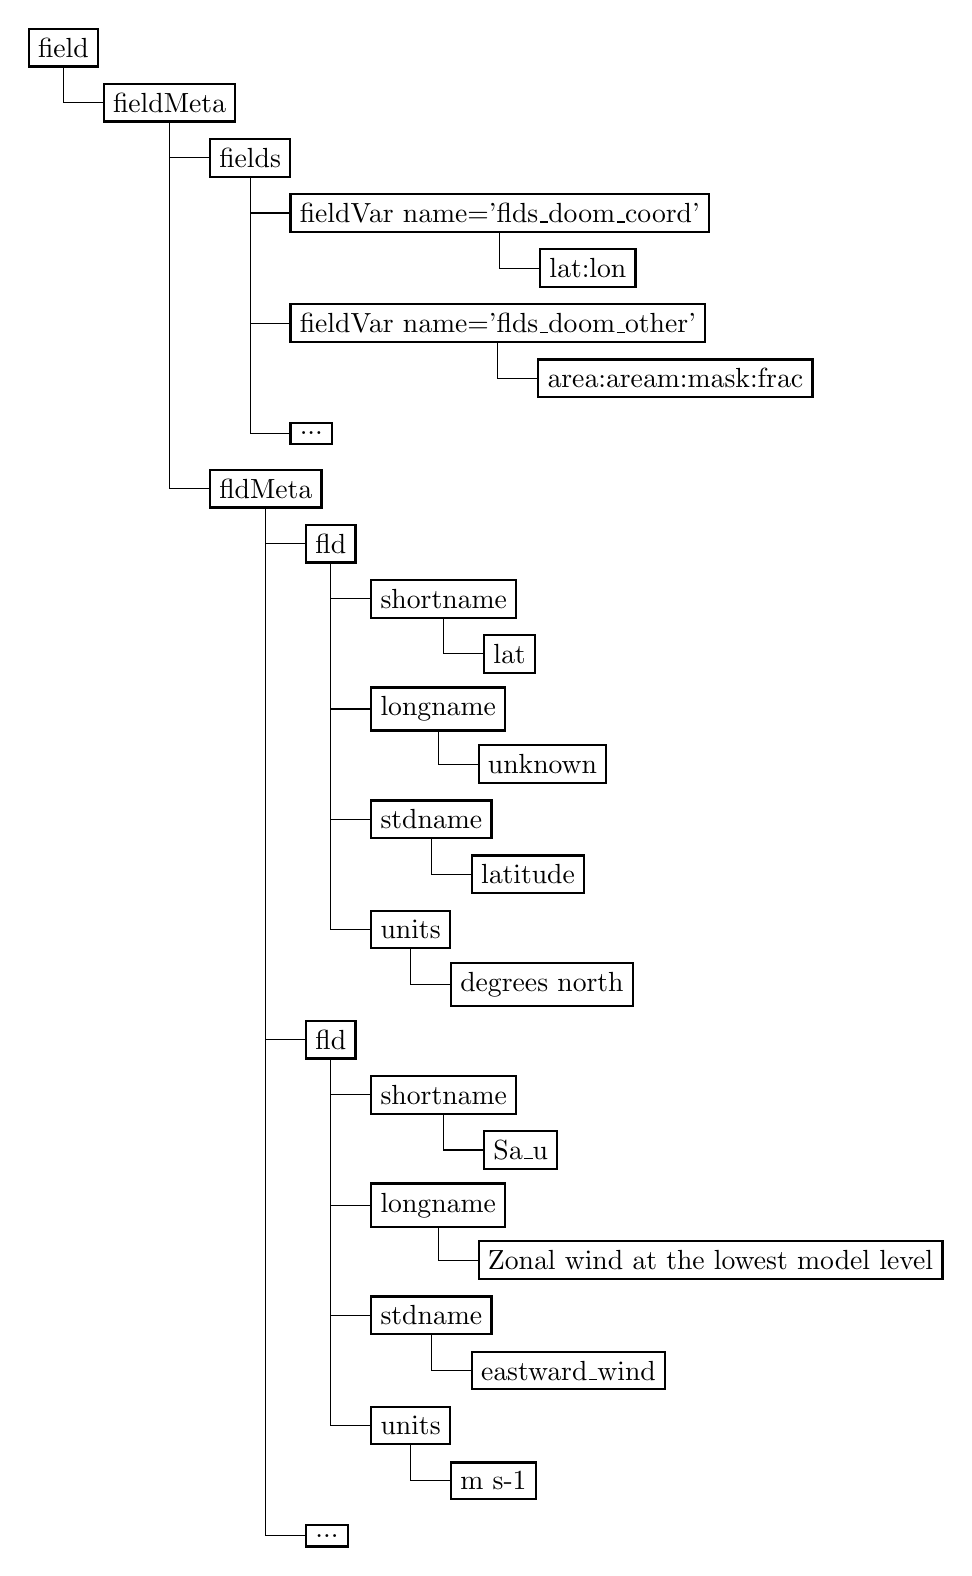
\begin{tikzpicture}[%
  grow via three points={one child at (0.5,-0.7) and
  two children at (0.5,-0.7) and (0.5,-1.4)},
  edge from parent path={(\tikzparentnode.south) |- (\tikzchildnode.west)}]

  \node{field}
  child { node {fieldMeta}
  child { node {fields}
    child { node {fieldVar name='flds\_doom\_coord'}
    	child { node {lat:lon} }
    }
    child [missing] {}
    child { node {fieldVar name='flds\_doom\_other'}
    	child { node {area:aream:mask:frac} }
    }
    child [missing] {}
    child { node {...} }
  }
  child [missing] {}
  child [missing] {}
  child [missing] {}
  child [missing] {}
  child [missing] {}
  child { node {fldMeta}
    child { node {fld}
      child { node {shortname}
        child {node {lat}}
      }
      child [missing] {}
      child { node {longname}
        child {node {unknown}}
      }
      child [missing] {}
      child { node {stdname}
        child {node {latitude}}
      }
      child [missing] {}
      child { node {units}
        child {node {degrees north}}
      }
      child [missing] {}
    }
    child [missing] {}
    child [missing] {}
    child [missing] {}
    child [missing] {}
    child [missing] {}
    child [missing] {}
    child [missing] {}
    child [missing] {}
    child { node {fld}
      child { node {shortname}
        child {node {Sa\_u}}
      }
      child [missing] {}
      child { node {longname}
        child {node {Zonal wind at the lowest model level}}
      }
      child [missing] {}
      child { node {stdname}
        child {node {eastward\_wind}}
      }
      child [missing] {}
      child { node {units}
        child {node {m s-1}}
      }
      child [missing] {}
    }
    child [missing] {}
    child [missing] {}
    child [missing] {}
    child [missing] {}
    child [missing] {}
    child [missing] {}
    child [missing] {}
    child [missing] {}
    child { node {...}}
  }
  };
\end{tikzpicture}